\documentclass[11pt,letterpaper]{article}

\newtheorem{theorem}{Theorem}
\newtheorem{corollary}{Corollary}
\newtheorem{lemma}{Lemma} 
\newtheorem{claim}{Claim}
\newtheorem{fact}{Fact}
\newtheorem{definition}{Definition}
\newtheorem{assumption}{Assumption}
\newtheorem{observation}{Observation}
\newtheorem{example}{Example}

\usepackage{epsfig}
\usepackage{graphicx}
\usepackage{amsmath}
\usepackage{amssymb}
\usepackage{enumerate}
\usepackage[margin=0.75in]{geometry}

\oddsidemargin 0in
\evensidemargin 0in
\textwidth 6.5in
\topmargin -0.5in
\textheight 9.0in
\abovecaptionskip 0in

\def\@maketitle
   {
   \newpage
   \null
   \vskip .375in
   \begin{center}
      {\Large \bf \@title \par}
      % additional two empty lines at the end of the title
      \vspace*{24pt}
      {
      \large
      \lineskip .5em
      \begin{tabular}[t]{c}
         \ifcvprfinal\@author\else Anonymous CVPR submission\\
         \vspace*{1pt}\\%This space will need to be here in the final copy, so don't squeeze it out for the review copy.
Paper ID \cvprPaperID \fi
      \end{tabular}
      \par
      }
      % additional small space at the end of the author name
      \vskip .5em
      % additional empty line at the end of the title block
      \vspace*{12pt}
   \end{center}
   }

\def\abstract
   {%
   \centerline{\large\bf Abstract}%
   \vspace*{12pt}%
   \it%
   }

\def\endabstract
   {
   % additional empty line at the end of the abstract
   \vspace*{12pt}
   }


\begin{document}
%%%%%%%%% TITLE
\title{{CS224W Course Project Proposal \\} \bf De-anonymizing social networks via network alignment}

\author{Danqi Chen\\
Stanford University\\
{\tt\small danqi@stanford.edu}
% For a paper whose authors are all at the same institution,
% omit the following lines up until the closing ``}''.
% Additional authors and addresses can be added with ``\and'',
% just like the second author.
% To save space, use either the email address or home page, not both
\and
Botao Hu\\
Stanford University\\
{\tt\small botaohu@stanford.edu}
%
\and
Shuo Xie\\
Stanford University\\
{\tt\small shuoxie@stanford.edu}
}

\maketitle
\thispagestyle{empty}

\maketitle

\section{Introduction}


With the booming and developing of online social media in recent years, a large amount of valuable social network data has been generated. Social network data are mined for a variety of purposes, businesses leverage data to learn about consumers in order to tailor and enhance experiences, government agencies rely on data to assess public opinions and formulate optimal policies, and scientists use data to study complex interpersonal interactions. 
As a standard way of privacy control, social network data are usually anonymized in order to be shared with third parties, i.e. names, address and demographical information are removed from the data set. However, anonymity is often misrepresented as sufficient to avoid privacy risks. Actually, with easy access to abundant publicly available auxiliary information, especially the social network connection structure, we may still identify individual users and thus de-anonymize social network data.
Social network de-anonymization is essentially a network alignment task, i.e., aligning an anonymized network to an identified network. However, existing de-anonymization algorithms \cite{Narayanan2009} adopt simple greedy based approach, without referring to the findings in the well studied field of network alignment. In this project, our group aims at performing social network de-anonymization via network alighnment method. In light of our works, we hope to redefine people's understanding of privacy protection, and contribute to the formulation of efficient government policies regarding privacy protection and re-evaluation of business practices surrounding the sharing of social-network data.


\section{Literature Review}

\subsection{De-anonymizing Social Networks}

Formally, the problem of de-anonymizing social networks is to identify the same users between two anonymized social networks.  A social network can be modeled as a directed graph (e.g., Twitter, Flickr) or an undirected graph (e.g., Facebook): Each node in the graph represents a user in the social network and each edge between two nodes characterizes the relationship between the users, such as ``following'' in Twitter or ``friendship'' in Facebook. In addition, anonymized graphs are usually released with at least some attributes in their nodes such as user profile information, user interests, corresponding to a set of attributes for each node in $V$, which may help us make de-anonymization easier.

\cite{Narayanan2009} is the first work to perform large-scale de-anonymization of real-world social networks. Specifically, they try to match the users between Twitter and Flickr and show that $30.8\%$ of the verifiable members of both social networks could be recognized with $12\%$ error rate. In their paper, they propose a greedy-based de-anonymization algorithm, which consists of two steps - ``seed finding'' and ``propagation''. In the ``seed finding'' step, they identify a small number of ``seed'' nodes which are present in the both networks and map them to each other; Later they use the seed nodes as ``anchors'' to propagate the de-anonymization to more and more nodes. They iteratively try to extend the mapping as follows: pick an arbitrary unmapped node in a graph, and map it to the ``most similar'' node in the other graph, where the similarity score is computed based on some heuristics such as cosine similarity or the number of formed squares.

It is worth noting that \cite{Narayanan2011} won the Kaggle Social Network Challenge by applying the above de-anonymizing algorithm to the contest dataset and real Flickr network, and exploit the connectivity among ``matched users'' in Flickr to perform link predictions. 

Although the proposed algorithm demonstrates the feasibility of successful de-anonymization on large-scale social networks, the algorithm is based on simple greedy approaches, so that the result is far from ``perfect matchings''; Furthermore, it is purely based on the network topology and doesn't take advantage of any attribute of nodes, and these public attributes may greatly improve the de-anonymization process.

\subsection{Network Alignment}
Network alignment is another well-formed problem, which aims to perform matchings or alignments between the vertices of two undirected graphs. This problem has been studied extensively, and has been applied successfully in many domains such as finding common pathways in biological networks(\cite{Singh2007, Singh2008, Liao2009}), ontology matchings between the Library of Congress with the categories from Wikipedia(\cite{Bayati2009}), and multi-lingual ontologies(\cite{Kreitmann2011, Bayati2009a}). In this subsection, we will review the existing algorithms that produce good solutions for the network alignment, analyze the strengths and weakness of these algorithms and finally investigate the possibility of applying network alignment algorithms on our settings of de-anonymizing social networks.
 
Most existing works formulate the network alignment problem as follows: given two sets of vertices $V_A = \{1, 2, \ldots, n\}, V_B = \{1', 2', \ldots, m'\}$, and $A = (V_A, E_A), B = (V_B, E_B)$ are two undirected graphs with their respective vertex and edge sets. Let $L$ be a bipartite graph between the vertices of $A$ and $B$, formally $L = (V_A \cup V_B, E_L)$ (in many algorithm settings, $L$ is the complete bipartite graph). The goal is to find a matching $M$ between $V_A$ and $V_B$ using only edges from $L$ ($M \subseteq L$), such that the number of overlapped edges is maximized. Here an edge $(i, j) \in E_A$ is \textit{overlapped} iff. $(i', j') \in E_B, (i, i')$ and $(j, j')$ belong to $M$.


\begin{figure}[!h]
\begin{center}
\includegraphics[scale = 0.5]{fig/matching}
\caption{The Network Alignment Problem}
\end{center}
\end{figure}

In a more general setting following \cite{Singh2007}, each edge $e \in E_L$ has a non-negative weight $w_e$, and the goal is to find a matching $M$ maximizing a linear combination of the matching weight and the number of over-lapped edges. Mathematically, it can be formulated as a quadratic program(QP): define $\mathbf{S}$ as a 0-1 matrix of size $|E_L| \times |E_L|$ where $S[ii',  jj'] = 1$ if $(i, j) \in E_A$ and $(i', j') \in E_B$, $\mathbf{A}$ as the binary incidence matrix of $L$ with dimensions $|V_L| \times |E_L|$. We want to find a 0-1 vector $\mathbf{x}$ such that:
\begin{eqnarray*}
		\max_{\mathbf{x}} & & {\alpha \mathbf{w}^{\intercal}\mathbf{x} + \beta \mathbf{x}^{\intercal}\mathbf{S}\mathbf{x}} \\
		\text{ subject to  } & &  \mathbf{A}\mathbf{x} \leq \mathbf{1}, x_{ii'} \in \{0, 1\}
\end{eqnarray*}

Solving the QP formulation is NP-hard, therefore many existing works have been attempted to relax the constraints or find the heuristics:

\textbf{IsoRank}(\cite{Singh2008}) learns a similarity measure $r_{ii'}$ between node $i$ in $V_A$ and node $i'$ in $V_B$ and $r_{ii'}$ is defined as:
	\begin{equation*}
           r_{ii'} = \sum_{(i, j) \in E_A}{\sum_{(i', j') \in E_B}{\frac{R_{j, j'}}{|N_j||N_{j'}|}}}.
	\end{equation*}
The new weights $r_{ii'}$ can be found using an eigen-value calculation as in PageRank. Later, \cite{Bayati2009a} proposes an extension of IsoRank algorithm based on the Kronecker product, named \textbf{SpaIsoRank}, which can be adapted to the case when $L$ is sparse. \cite{Kollias2011} proposes a \textbf{Network Similarity Decomposition (NSD)} algorithm, which uses matrix decomposition to approximate the power iteration in IsoRank and runs much faster than the original algorithm.

\cite{Klau2009} formulates a \textbf{linear programming(LP)} relaxation of the original QP, and proposes an iterative approximation algorithm, which is a tigher LP relaxation and Lagrangian decomposition of the symmetry constraints. This algorithm can be used to handle large networks when $L$ is sparse.

\cite{Bayati2009a} proposes two message passing algorithms \textbf{MP} and \textbf{MP++} for network alignment: It constructs a fractor graph and defines a probability distribution on the space of all matchings in $L$ that assigns the highest probability to the matching that maximize the QP, and then applies the stanford Belief Progapation algorithm for finding the optimum solution. As well, MP algorithms can be applied to large sparse networks.

In last year's course project \cite{Kreitmann2011}, Kreitmann proposes a simple \textbf{simulated annealing(SA)} algorithm, which initializes a greedy-based matching first, and adopts simulated algorithm approach taking the number of ``overlapped'' edges as the heuristic function for swapping two matches. 

Although the above algorithms may produce good results in their applications, we still have some concerns:
\begin{itemize}
	\item
		To our knowledge, no network alignment algorithm has been applied to the problem of de-anonymizing social network.
	\item
		IsoRank, LP, and MP algorithms can only be applied in small networks (e.g., biological networks) or large-scale sparse networks. For handling large-scale networks, how to select $L$ should be an issue we need to consider. 
	\item
		All the network alignment algorithms are based only on the network structure, no node attribute is considered to improve the alignment. 
	\item
		All the above algorithms are applying to aligning two undirected networks, we should consider if it is possible to develop network alignment algorithms for two directed network or one undirected network and one directed network, which can be adopted to our social networks such as Twitter and Flickr. 
\end{itemize}


\section{Proposal}

Generally speaking, our goal of this course project is to develop algorithms for de-anonymizing real-world social networks. 
\begin{itemize}
	\item
		We will crawl three online social networks by ourselves including the social network structure and the data of user profiles, and also build the ground truth via some other Web resources for evaluation. We will introduce this part in Subsection \ref{datasection}.
	\item
		We will try to adopt state-of-the-art network alignment algorithms on our de-anonymizing social network settings, as well compare with the greedy-based approaches in \cite{Narayanan2009}. We expect to deeply investigate the problem and perform intensive comparisons, and finally reach a satisfying solution. Details will be introduced in Subsection \ref{methodsection}.
\end{itemize}

\subsection{Data \& Evaluation}
\label{datasection}
We will use the data from three large online social networks in our experiments: Twitter, Flickr and Foursquare. On these social networks, the data of user profiles and friendship connections are all public and accessable by crawlers or APIs. 

The first graph is the ``following'' relationships on the Twitter\footnote{http://www.twitter.com}, a microblogging service, which has 500 million users (200 million active). We consider to adopt the data crawled  on July 2009 by Kwak et al. \footnote{http://an.kaist.ac.kr/traces/WWW2010.html} containing 41 million users. In order to increase the overlap to the other two social networks, we will crawl more and extend this dataset to the latest network as possible. 
The second graph is the ``contact'' relationship on Flickr\footnote{http://www.flickr.com}, a photo-sharing service, which has 51 million registered members and 6 billion images on Jan 19, 2012.
The third graph is the ``Friends'' relationships on Foursquare\footnote{http://www.foursquare.com}, a location-based social network, which has 22 million global users on March 2, 2012. 


\subsubsection{Ground truth}

To verify our de-anonymizing results , we have to determine the ground truth, i.e., the true mapping between the users of the online social networks. Actually, we do not need to label the mapping of all users since the ground truth as a test set can be far smaller than the complete network data.
Instead of labeling the user mapping by human editors, there are several sources to get the ground truth. 

\begin{itemize}
\item
About.me\footnote{http://about.me} is a personal web hosting service, which had at least 1 million users on October, 2011 \footnote{http://techcrunch.com/2011/10/17/about-mes-ceo-on-how-to-hit-a-million-users-in-300-days-figure-out-who-your-entourage-is/}. The site offers registered users a simple platform to link multiple online identities, relevant external sites, and popular social networking websites such as Google+, Twitter, Facebook, LinkedIn, Flickr, YouTube, Foursquare. These links on user profile is actually human-labelled mapping generated by users themselves, which can be seen as a non-error ground truth.  We randomly sampled a portion of the mappings and verified by human inspection that most of about.me users have Twitter accounts and at least one of Flickr and Foursquare accounts. About.me also provides simple APIs to list user directory and view the links on user profile without the strict crawling limitation. Therefore, basically we will adopt the data from about.me to be our ground truth in this project.
\item
The links of the user profile pages on the social networking websites are another great source for ground truth, which are also user-generated. Usually, an individual user has many accounts for different social networking websites. On the user profile page, there might be links to this user's accounts on other popular social networking webistes. Especially, it has now been a standard practice for users to log into other social networking websites via his/her Twitter or Facebook account, and that website may show the user's Twitter and Facebook account in the user profile. For example, the figure \ref{fig:infer} shows how the links connect to other social networking websites on the user profile page among the famous large social networking website: LinkedIn publicly shows the users' linked Twitter account and Gmail/Google+ account; and public Google+ profile reveals the user's Facebook and Twitter account; and Foursquare will show the user's login Twitter or Facebook account information. 

\begin{figure}[h!]
\centering
\caption{Links on the user profile page of serveral social networking website}
\label{fig:infer}
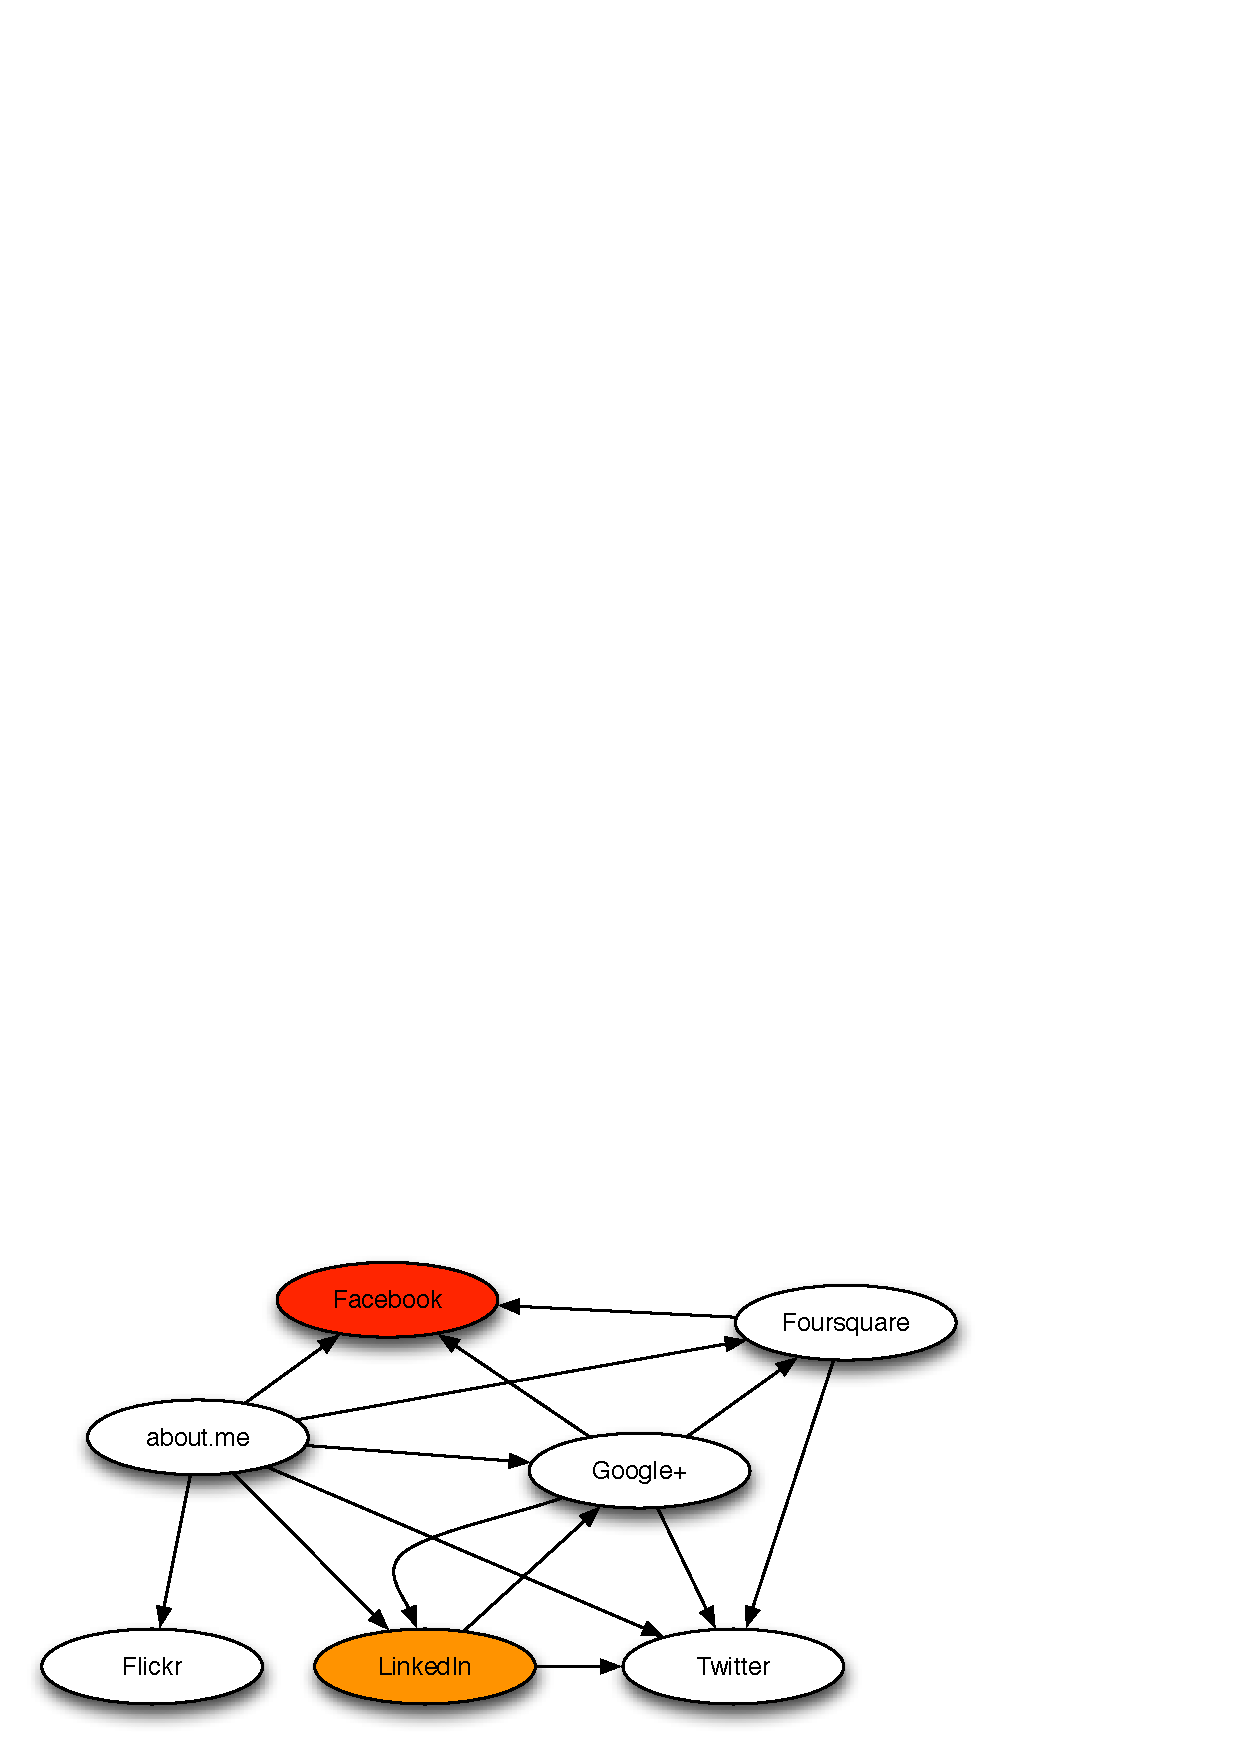
\includegraphics[width=0.7\textwidth]{fig/infer.jpg}
\end{figure}

Fortunately, on these famous social networking webistes in the figure \ref{fig:infer}, the most of user's profile pages are publicly accessbile. A crawler can easily follow these links on the profile page, discover all linked accounts about one user, and even retrieve the user's real name and affiliation from the profile on the real-name social networking website, such as LinkedIn and Facebook (colorred in orange and red in figure \ref{fig:infer}. Thus, we can build a ground truth by exploring all linked accounts of each user. 

\end{itemize}


Narayanan at el. \cite{Narayanan2008} did the experiment on aligning Twitter and Flickr data. However, they use an approximate ground truth: the similar username in the different networks. As their report claims, they  verified sample of mappings by human inspection that the error rate is around 5\%. We will replace their ground truth with our zero-error ground truth.

\subsubsection{Evaluation}
After collecting datasets and their ground truth, we will compare and evaluate algorithms on our datasets based on:
\begin{itemize}
\item
Accurary: Given a ground truth, the accurary evaluation can be simply the correct matches between two networks. 
\item
Scalability: Running time on the large-scale data.
\end{itemize}

\subsection{Methods}
\label{methodsection}
We plan to implement and compare several algorithms for de-anonymizing social networks:
\begin{itemize}
	\item
		Greedy algorithm  \cite{Narayanan2009}
	\item
		IsoRank \cite{Singh2007}
	\item 
		Linear Programming algorithm(LP) \cite{Klau2009}
	\item
		Message Passing algorithm(MP) \cite{Bayati2009a,Pache2012}
	\item
		Simulated Annealing \cite{Kreitmann2011}
\end{itemize}
In our project, we may need to consider the following questions:
\begin{itemize}
	\item
		For the network alignment algorithms such as IsoRank, LP and MP, how could we constrain the possible matching set $L$? Possibly, we could compute $L$ according to the similarity based on the attributes of nodes. And, how large of $L$ could be that these algorithms can be successfully applied?
	\item
		How could we apply the algorithms for aligning undirected networks on our directed network settings?
	\item
		Is it possible to develop other better (randomized) heuristic algorithms, incorporate with the node attributes?
\end{itemize}

\section{Deliverable}
\begin{itemize}
\item
We will provide a new dataset for network alignment on the large social networking website and also a sufficient number of zero-error ground truth. 

\item We will propose a novel algorithm which concerns the questions in Section \ref{methodsection}.

\item
We will submit a report of the empirical comparison of several algorithms on the real-world large-scale datasets. 

\item
We will implement most of the codes in SNAP\footnote{http://snap.stanford.edu} framework and integrate some complete componments of network alignment into the SNAP package.  
\end{itemize}
\bibliographystyle{abbrv}
\bibliography{na}

\end{document}
